\chapter{Neutrino Oscillation Physics}
\label{chap:NeutrinoOscillationPhysics}

When first proposed, neutrinos were expected to be massless fermions that only interact through weak and gravitational forces. This meant they were very difficult to detect as they can pass through significant amounts of matter without interacting. Despite this, experimental neutrino physics has developed with many different detection techniques and neutrino sources being used today. In direct tension with \ChangeOneRM{the} standard model physics, neutrinos have been determined to oscillate between different lepton flavours, requiring them to have mass.

\ChangeOne{The observation techniques which lead to the discovery of the neutrino are documented in \autoref{sec:NeutrinoOscillationPhysics_Discovery}}. The theory underpinning neutrino oscillation is described in \autoref{sec:NeutrinoOscillationPhysics_EvidenceForNeutrinoOscillation} \ChangeOneRM{. This section} \ChangeOne{and} includes the approximations which can be made to simplify the understanding of neutrino oscillation in \ChangeOneRM{a} \ChangeOne{the} two-flavour approximation \ChangeOneRM{as well as how the medium in which neutrinos propagate can manipulate the oscillation probability}. \ChangeOne{The past} \ChangeOne{Past}, current, and future neutrino experiments are detailed in \autoref{sec:NeutrinoOscillationPhysics_OscillationMeasurements}, including the reactor, atmospheric, and long-baseline accelerator neutrino sources that have been used to successfully constrain oscillation \ChangeOne{parameters} \ChangeOneRM{determination}. \ChangeOne{Finally, the current state of oscillation parameter measurements are summarised in \autoref{sec:Theory_Summary}.}

\section{Discovery of Neutrinos}
\label{sec:NeutrinoOscillationPhysics_Discovery}

At the start of the \quickmath{20^{th}} century, the electrons emitted from the \quickmath{\beta}-decay of the nucleus were found to have a continuous energy spectrum \cite{Chadwick:262756, Ellis1927-qf}. This observation seemingly broke the energy conservation invoked within that period's nuclear models.  Postulated in 1930 by Pauli as the solution to this problem, the neutrino (originally termed ``neutron'') was theorized to be an electrically neutral spin-\quickmath{1/2} fermion with a mass of the same order of magnitude as the electron \cite{Pauli:1930pc}. This neutrino was to be emitted with the electron in \quickmath{\beta}-decay to alleviate the apparent breaking of energy conservation. As a predecessor of \ChangeOneRM{the} \ChangeOne{today's} weak interaction model, Fermi's theory of \quickmath{\beta}-decay developed the understanding by coupling the four constituent particles; electron, proton, neutron, and neutrino, into a consistent model \cite{Fermi:1934hr}.

Whilst Pauli was not convinced of the ability to detect neutrinos\ChangeOne{, t}he first observations of the particle were made in the mid-1950s when neutrinos from a reactor were observed via the inverse \quickmath{\beta}-decay (IBD) process, \quickmath{\bar{\nu}_{e} + p \rightarrow n + e^{+}} \cite{reines_cowan_1,reines_cowan_2}.
%The detector consisted of cadium-doped water targets surronded by liquid scintillator, which was monitored by a suite of photo-multiplier tubes.
The detector consisted of two parts: a neutrino interaction medium and a liquid scintillator. The interaction medium was built from two water tanks. These were loaded with cadmium chloride to allow increased efficiency of neutron capture. The positron emitted from IBD annihilates, \quickmath{e^{+} + e^{-} \rightarrow 2\gamma}, generating a prompt signal and the neutron is captured on the cadmium via \quickmath{n + ^{108}Cd \rightarrow ^{109\ChangeOne{*}}Cd \rightarrow ^{109}Cd + \gamma}, producing a delayed signal. \ChangeOneRM{The experiment observed an increase in the neutrino event rate when the reactor was operating compared to when it was switched off, in much the same way as modern reactor neutrino experiments operate.} \ChangeOne{An increase in the coincidence rate was observed when the reactor was operating which was interpretted as interactions from neutrinos generated in the reactor.}

After the discovery of the \quickmath{\nu_{e}}, the natural question of how many flavours of neutrino exist was asked. In 1962, a measurement of the \quickmath{\nu_{\mu}} was conducted at the Brookhaven National Laboratory \cite{Lederman}. A proton beam was directed at a beryllium target, generating a \quickmath{\pi}-dominated beam which then decayed via \quickmath{\pi^{\pm} \rightarrow \mu^{\pm} + (\nu_{\mu}, \bar{\nu}_\mu}), and the subsequent interactions of the \quickmath{\nu_{\mu}} were observed. \ChangeOne{As the subsequent interaction of the neutrino geenerates muons rather than electrons, it was determined the \quickmath{\nu_{\mu}} was fundamentally different from \quickmath{\nu_{e}}.} The final observation to be made was that of the \quickmath{\nu_{\tau}} from the DONUT experiment \cite{tau_nu_disc}. Three neutrinos seem the obvious solution as it mirrors the known number of charged lepton (as they form weak isospin doublets) but there could be evidence of more. Several neutrino experiments have found anomalous results \cite{PhysRevD.64.112007, PhysRevLett.110.161801} which could be attributed to sterile neutrinos \ChangeOne{. However,} \ChangeOneRM{however} cosmological observations indicate the number of neutrino species \ChangeOne{\quickmath{N_{eff} = 2.99 \pm 0.17} \cite{Planck2018}, as measured from the cosmic microwave background power spectrum, and Stanford Linear Accelerator found the number of active neutrino flavours to be \quickmath{N_{\nu} 2.9840 \pm 0.0082} \cite{lep} from measurements of the Z-decay width.}

\section{Theory of Neutrino Oscillation}
\label{sec:NeutrinoOscillationPhysics_EvidenceForNeutrinoOscillation}

As direct evidence of beyond Standard Model physics, a neutrino generated with lepton flavour \quickmath{\alpha} can change into a different lepton flavour \quickmath{\beta} after propagating some distance. This phenomenon is called neutrino oscillation and requires that neutrinos must have a non-zero mass (as seen in \autoref{sec:NeutrinoOscillationPhysics_3FlavourOsc}). This \ChangeOne{observation} is direct evidence of beyond standard model physics. This behaviour has been characterised by the Pontecorvo-Maki-Nakagawa-Sakata (PMNS) \cite{p1,p2,km} mixing matrix which describes how the flavour and mass of neutrinos are associated. This is analogous to the Cabbibo-Kobayashi-Maskawa (CKM) \cite{cabbibo} matrix measured in quark physics.

\subsection{Three Flavour Oscillations}
\label{sec:NeutrinoOscillationPhysics_3FlavourOsc}

The PMNS parameterisation defines three flavour eigenstates, \quickmath{\nu_{e}}, \quickmath{\nu_{\mu}} and \quickmath{\nu_{\tau}} (indexed \quickmath{\nu_{\alpha}}), which are \ChangeOneRM{assigned based upon} \ChangeOne{eigenstates of} the weak interaction \ChangeOneRM{flavour states} and three mass eigenstates, \quickmath{\nu_{1}}, \quickmath{\nu_{2}} and \quickmath{\nu_{3}} (indexed \quickmath{\nu_{i}}). Each mass eigenstate is the superposition of all three flavour states,

\begin{equation}
  \label{eq:NeutrinoOscillationPhysics_Superposition}
  \left|\nu_{i}\right> = \sum_{\alpha}\mathrm{U}_{\alpha i}\left|\nu_{\alpha}\right>.
\end{equation}

\ChangeOne{Where} \quickmath{\mathrm{U}} is the PMNS matrix which \ChangeOne{is unitary and connects} \ChangeOneRM{correlates} the mass and flavour eigenstates.

%
\iffalse
\begin{equation}
  \label{eq:NeutrinoOscillationPhysics_PMNSReduced}
  \mathrm{U} = \begin{pmatrix} \mathrm{U}_{e1} & \mathrm{U}_{e2} & \mathrm{U}_{e3} \\ \mathrm{U}_{\mu 1} & \mathrm{U}_{\mu 2} & \mathrm{U}_{\mu 3} \\ \mathrm{U}_{\tau 1} & \mathrm{U}_{\tau 2} & \mathrm{U}_{\tau 3} \end{pmatrix}.
\end{equation}
\fi
%

\ChangeOneRM{Neutrinos interact with leptons of the same weak flavour eigenstate rather than mass eigenstate.} \ChangeOne{The weak interaction couples to flavour eigenstates so neutrinos interact with leptons of the same flavour.} The propagation of a neutrino flavour eigenstate, in a vacuum, can be re-written as a plane-wave solution to the time-dependent Schr{\"o}dinger equation,

\begin{equation}
  \label{eq:NeutrinoOscillationPhysics_TimeDepSuperposition}
  \left|\nu_{\alpha}(t)\right> = \sum_{i}\mathrm{U}^{*}_{\alpha i}\left|\nu_{i}\right>e^{-i \phi_{i}}.
\end{equation}

The probability of observing a neutrino of flavour eigenstate \quickmath{\beta} from one which originated as flavour \quickmath{\alpha} can be calculated as,

\begin{equation}
  \label{eq:NeutrinoOscillationPhysics_ProbabilityComplexForm}
  P(\nu_{\alpha} \rightarrow \nu_{\beta}) = \left| \left< \nu_{\beta} | \nu_{\alpha}(t) \right> \right|^{2} = \sum_{i,j} \mathrm{U}^{*}_{\alpha i}\mathrm{U}_{\beta i}\mathrm{U}_{\alpha j}\mathrm{U}^{*}_{\beta j} e^{-i(\phi_{j}-\phi_{i})}
\end{equation}

The \quickmath{\phi_{i}} term can be expressed in terms of the energy, \quickmath{E_{i}}, and magnitude of the three momenta, \quickmath{p_{i}}, of the neutrino, \quickmath{\phi_{i} = E_{i}t - p_{i}x} (\quickmath{t} and \quickmath{x} being time and position coordinates). Therefore,

\begin{equation}
  \label{eq:NeutrinoOscillationPhysics_PhaseDifference}
  \phi_{j}-\phi_{i} = E_{j}t - E_{i}t - p_{j}x + p_{i}x .
\end{equation}

For a relativistic particle, \quickmath{E_{i} \gg m_{i}},

\begin{equation}
  p_{i} = \sqrt{E^{2}_{i} - m^{2}_{i}} \approx E_{i} - \frac{m^{2}_{i}}{2E_{i}}.
\end{equation}

Making the approximations that neutrinos are relativistic, the mass eigenstates were created with the same energy and that \quickmath{x = L}, where \quickmath{L} is the distance traveled by the neutrino, \autoref{eq:NeutrinoOscillationPhysics_PhaseDifference} then becomes

\begin{equation}
  \phi_{j}-\phi_{i} = \frac{\Delta m^{2}_{ij} L}{2E},
\end{equation}

where \quickmath{\Delta m^{2}_{ij} = m^{2}_{i} - m^{2}_{j}}. This, \ChangeOneRM{teamed} \ChangeOne{combined} with further use of unitarity relations results in \autoref{eq:NeutrinoOscillationPhysics_ProbabilityComplexForm} becoming

\begin{equation}
  \label{eq:NeutrinoOscillationPhysics_ProbabilityComplexForm2}
  P(\nu_{\alpha} \rightarrow \nu_{\beta}) = \delta_{\alpha \beta} - 4 \sum_{i>j} \mathbb{R} \left( \mathrm{U}^{*}_{\alpha i}\mathrm{U}_{\beta i}\mathrm{U}_{\alpha j}\mathrm{U}^{*}_{\beta j} \right) \sin^{2} \left( \frac{\Delta m^{2}_{ij} L}{4E} \right) \\ + \left( - \right) 2 \sum_{i>j} \mathbb{I} \left( \mathrm{U}^{*}_{\alpha i}\mathrm{U}_{\beta i}\mathrm{U}_{\alpha j}\mathrm{U}^{*}_{\beta j} \right) \sin \left( \frac{\Delta m^{2}_{ij} L}{2E} \right) \notag.
\end{equation}

Where \quickmath{\delta_{\alpha \beta}} is the Kronecker delta function and the negative sign \ChangeOne{on the last term} is included for the oscillation probability of antineutrinos.

Typically, the PMNS matrix is parameterised into three mixing angles, a charge parity (CP) violating phase \quickmath{\delta_{CP}}, and two Majorana phases \quickmath{\alpha_{1,2}},

\begin{equation}
  \label{eq:NeutrinoOscillationPhysics_PMNS}
  \mathrm{U} =
  \underbrace{\begin{pmatrix} 1 & 0 & 0 \\ 0 & c_{23} & s_{23} \\ 0 & -s_{23} & c_{23} \end{pmatrix}}_{\text{Atmospheric, Accelerator}}
  \underbrace{\begin{pmatrix} c_{13} & 0 & s_{13}e^{-i \delta_{CP}} \\ 0 & 1 & 0 \\ -s_{13}e^{-i \delta_{CP}} & 0 & c_{13} \end{pmatrix}}_{\text{Reactor, Accelerator}}
  \underbrace{\begin{pmatrix} c_{12} & s_{12} & 0 \\ -s_{12} & c_{12} & 0 \\ 0 & 0 & 1 \end{pmatrix}}_{\text{Reactor, Solar}}
  \underbrace{\begin{pmatrix} e^{i\alpha_{1}/2} & 0 & 0 \\ 0 & e^{i\alpha_{2}/2} & 0 \\ 0 & 0 & 1 \end{pmatrix}}_{\text{Majorana}}.
\end{equation}

Where \quickmath{s_{ij} = \sin(\theta_{ij})} and \quickmath{c_{ij} = \cos(\theta_{ij})}. The oscillation parameters are often grouped; \quickmath{(1,2)} as ``solar'', \quickmath{(2,3)} as ``atmospheric'' and \quickmath{(1,3)} as ``reactor''. Many neutrino experiments aim to measure the PMNS parameters from a wide array of origins, as is the purpose of this thesis.

The Majorana phase, \quickmath{\alpha_{1,2}}, \ChangeOneRM{containing matrix} included within \ChangeOne{the fourth matrix in} \autoref{eq:NeutrinoOscillationPhysics_PMNS} is only included for completeness. For an oscillation analysis experiment, \ChangeOneRM{any term in this oscillation probability calculation containing this phase disappears} \ChangeOne{any terms containing thtis phase disappear} due to taking the expectation value of the PMNS matrix. \ChangeOne{Measurements of these phases are typically performed by experiments searching for neutrino-less double \quickmath{\beta}-decay \cite{Maio_2015}.}

A two flavour approximation can be \ChangeOneRM{attained} \ChangeOne{obtained} when one assumes the third mass eigenstate is degenerate with another. As discussed in \autoref{sec:NeutrinoOscillationPhysics_OscillationMeasurements}, it is found that \quickmath{\Delta m^{2}_{21} \ll |\Delta m^{2}_{31}|}. This results in the two flavour approximation being reasonable for understanding the features of the oscillation. In this two flavour case, the mixing matrix becomes,

\begin{equation}
  \label{eq:NeutrinoOscillationPhysics_PMNS_2Flavour}
  \mathrm{U_{\text{2 Flav.}}} = \begin{pmatrix} \cos(\theta) & \sin(\theta) \\ -\sin(\theta) & \cos(\theta) \end{pmatrix}.
\end{equation}

This culminates in the oscillation probability,

\begin{equation}
  \label{eq:NeutrinoOscillationPhysics_PMNS_2FlavourOscProb}
  \begin{split}
  P(\nu_{\alpha} \rightarrow \nu_{\alpha}) &= 1 - \sin^{2} \left( 2\theta \right) \sin^2 \left( \frac{\Delta m^{2} L}{4E} \right), \\
  P(\nu_{\alpha} \rightarrow \nu_{\beta}) &= \sin^{2} \left( 2\theta \right) \sin^2 \left( \frac{\Delta m^{2} L}{4E} \right).
  \end{split}
\end{equation}

\ChangeOneRM{For} \ChangeOne{Where} \quickmath{\alpha \neq \beta}. For a fixed neutrino energy, the oscillation probability is a sinusoidal function depending upon the distance over which the neutrino propagates. The frequency and amplitude of oscillation are dependent upon \ChangeOneRM{the ratio of the} \quickmath{\Delta m^{2} / 4E} and \quickmath{\sin^2{2\theta}}, respectively. \ChangeOne{The oscillation probabilities presented thus far assume \quickmath{c=1}, where \quickmath{c} is the speed of light in vacuum.} \ChangeOne{In more familiar units}, the maximum oscillation probability for a fixed value of \quickmath{\theta} is given at \quickmath{L[km]/E[GeV] \sim 1.27 / \Delta m^{2}}. It is this calculation that determines the best \quickmath{L/E} value for a given experiment to be designed around for measurements of a specific value of \quickmath{\Delta m^{2}}.

\subsection{The MSW Effect}
\label{sec:NeutrinoOscillationPhysics_MSW}

The theory of neutrino oscillation in a vacuum \ChangeOneRM{is} \ChangeOne{has been} described in \autoref{sec:NeutrinoOscillationPhysics_3FlavourOsc}. However, the beam neutrinos and atmospheric neutrinos originating from below the horizon propagate through matter in the Earth. The coherent scattering of neutrinos from a material target modifies the Hamiltonian of the system. This results in a change in the oscillation probability. Notably, charged current scattering (\quickmath{\nu_{e} + e^{-} \rightarrow \nu_{e} + e^{-}}, propagated by a \quickmath{W} boson) only affects electron neutrinos \ChangeOneRM{compared to} \ChangeOne{whereas} the neutral current scattering (\quickmath{\nu_{l} + l^{-} \rightarrow \nu_{l} + l^{-}}, propagated by a \quickmath{Z^{0}} boson) interacts through all neutrino flavours equally. In the two-flavour \ChangeOneRM{limit} \ChangeOne{approximation}, the effective mixing parameter becomes

\begin{equation}
  \label{eq:NeutrinoOscillationPhysics_2Flavour_MSW}
  \sin^{2}(2\theta) \rightarrow \sin^{2}(2\theta_{m}) = \frac{\sin^{2}(2\theta)}{(A/\Delta m^{2} - \cos(2\theta))^{2} + \sin^{2}(2\theta)},
\end{equation}

where \quickmath{A = 2\sqrt{2}G_{F}N_{e}E}, \ChangeOneRM{with} \quickmath{N_{e}} is the electron density of the medium and \quickmath{G_{F}} is Fermi's constant. It is clear to see that there exists a value of \quickmath{A = \Delta m^{2} \cos(2\theta)} for \quickmath{\Delta m^{2} > 0} which results in a divergent mixing parameter. This resonance is \ChangeOneRM{due to} \ChangeOne{termed} the Mikheyev-Smirnov-Wolfenstein (MSW) effect (or more colloquially, the matter resonance) which regenerates the electron neutrino component of the neutrino flux \cite{Smirnov2003-yb, msw, wolfenstein}. The density at which the resonance occurs is given by

\begin{equation}
  \label{eq:NeutrinoOscillationPhysics_ResonanceDensity}
  N_{e} = \frac{\Delta m^{2} \cos(2\theta)}{2\sqrt{2} G_{F} E}.
\end{equation}

At densities lower than this critical value, the oscillation probability will be much closer to that of vacuum oscillation. \ChangeOne{For antineutrinos, \quickmath{N_{e} \rightarrow -N_{e}} \cite{Barger:1980tf}.} The resonance occurring from the MSW effect depends on the sign of \quickmath{\Delta m^{2}}. Therefore, any neutrino oscillation experiment which observes neutrinos and antineutrinos which have propagated through matter can have some sensitivity to the ordering of the neutrino mass eigenstates.

\section{Neutrino Oscillation Measurements}
\label{sec:NeutrinoOscillationPhysics_OscillationMeasurements}

As evidence of beyond standard model physics, the 2015 Nobel Prize in Physics was awarded to the Super-Kamiokande (SK) \cite{PhysRevLett.93.101801} and Sudbury Neutrino Observatory (SNO) \cite{PhysRevLett.89.011301} collaborations for the first definitive observation of solar and atmospheric neutrino oscillation \cite{2015NobelPhysicsPrize}. Since then, the field has seen a wide array of oscillation measurements from a variety of neutrino sources. As seen in \autoref{sec:NeutrinoOscillationPhysics_3FlavourOsc}, the neutrino oscillation probability is dependent on the ratio of the propagation baseline, \quickmath{L}, to the neutrino energy, \quickmath{E}. It is this ratio that determines the type of neutrino oscillation a particular experiment is sensitive to.

As illustrated in \autoref{fig:NeutrinoOscillationPhysics_EnergySpectrum}, there are many neutrino sources that span a wide range of energies. The least energetic neutrinos are from diffuse supernovae and terrestrial neutrinos at \quickmath{O(1)\text{MeV}} whereas the most energetic neutrinos originate from atmospheric and galactic neutrinos of \quickmath{>O(1)\text{TeV}}.

\begin{figure}[h]
  \begin{subfigure}[t]{0.95\textwidth}
    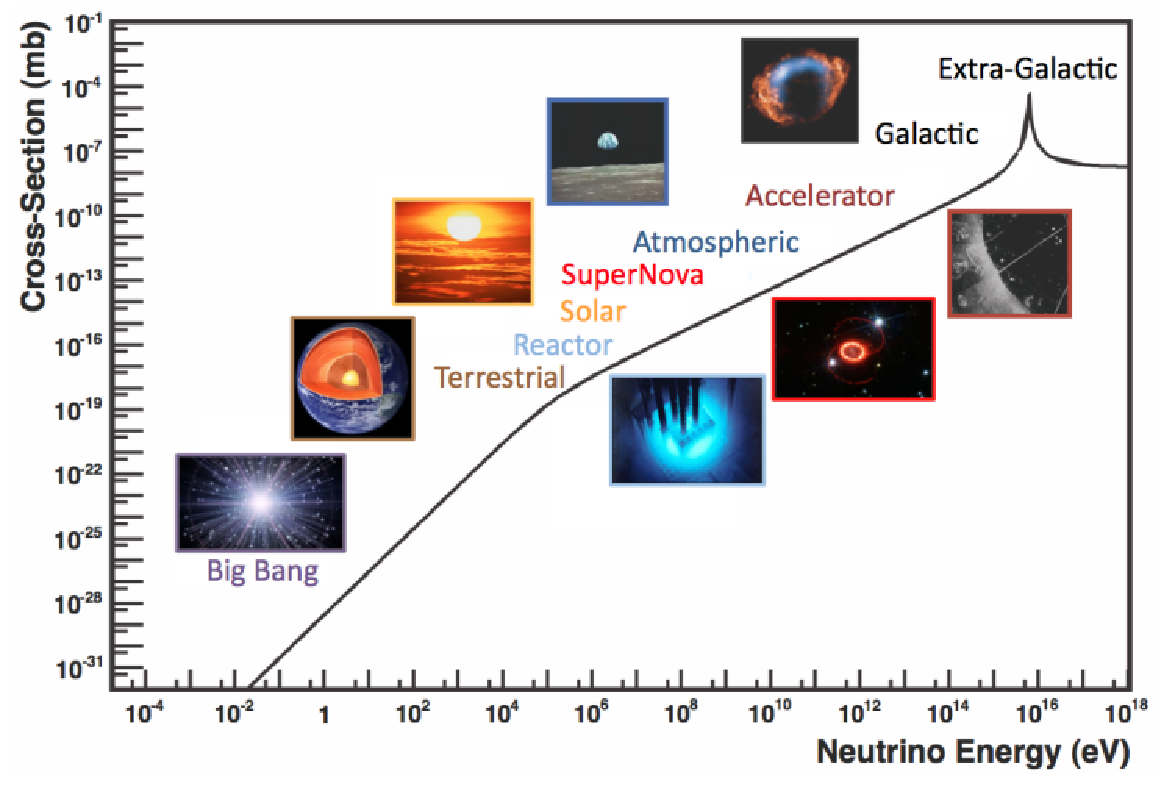
\includegraphics[width=\textwidth, trim={0mm 0mm 0mm 0mm}, clip,page=1]{Figures/Theory/EnergySpectrum.pdf}
  \end{subfigure}
  \caption{The cross-section of neutrinos from various natural and man-made sources as a function of neutrino energy. Taken from \cite{Formaggio:2012cpf}}
  \label{fig:NeutrinoOscillationPhysics_EnergySpectrum}
\end{figure}

\subsection{Solar Neutrinos}
\label{subsec:NeutrinoOscillationPhysics_SolarNeutrinos}

Solar neutrinos are emitted from fusion reaction chains at the center of the Sun. The solar neutrino flux, given as a function of neutrino energy for different fusion and decay chains, is illustrated in \autoref{fig:NeutrinoOscillationPhysics_SolarNeutrinoFlux}. Whilst proton-proton fusion generates the largest flux of neutrinos, the neutrinos are of low energy and are difficult to reconstruct due to the IBD interaction threshold of \quickmath{1.8\text{MeV}}. Consequently, most experiments focus on the neutrinos from the decay of \quickmath{^{8}B} (via \quickmath{^{8}B \rightarrow ^{8}Be^{*} + e^{+} + \nu_{e}}), which are higher energy.

\begin{figure}[h]
  \begin{subfigure}[t]{0.80\textwidth}
    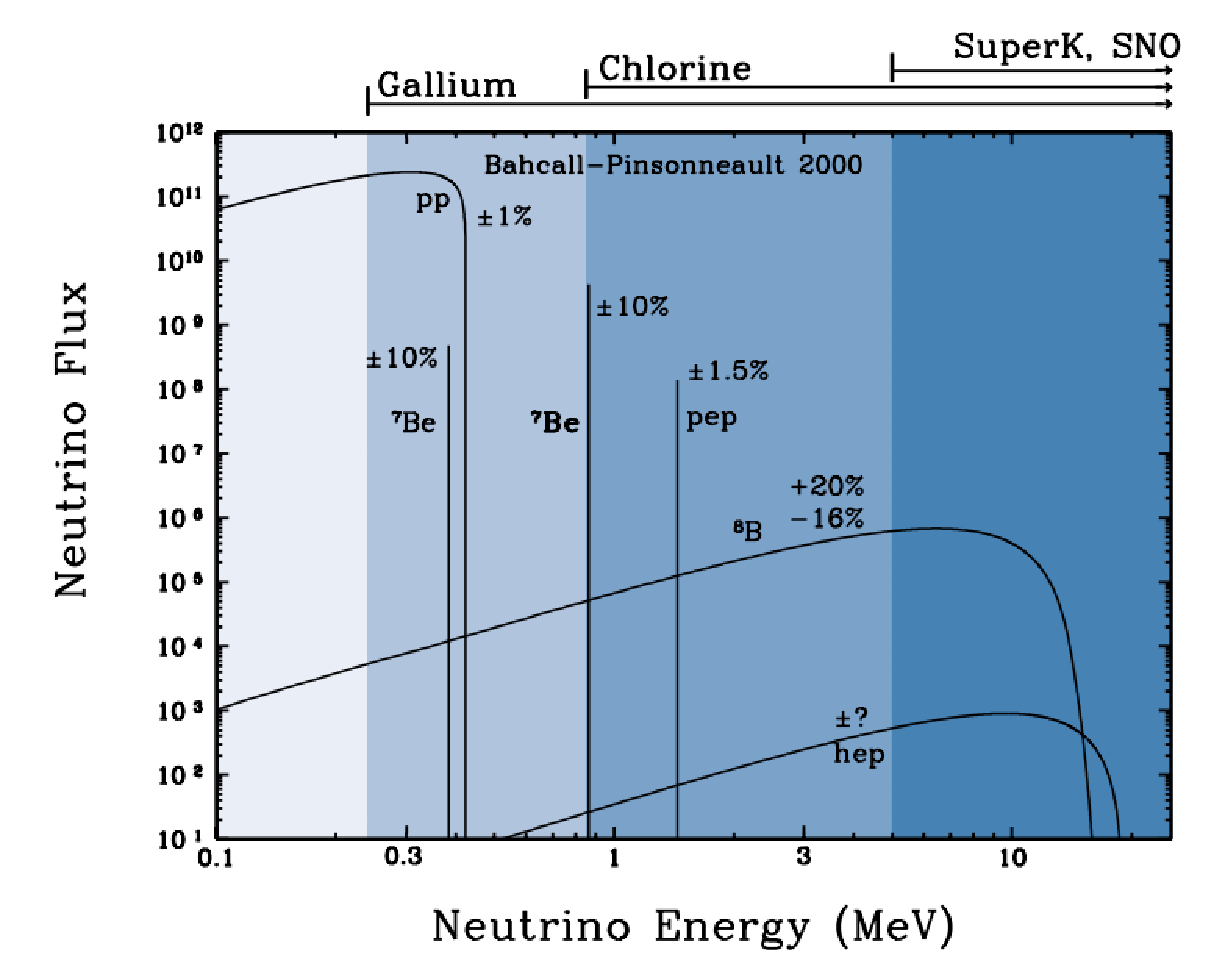
\includegraphics[width=\textwidth, trim={0mm 0mm 0mm 0mm}, clip,page=1]{Figures/Theory/SolarNeutrinoFlux.pdf}
  \end{subfigure}
  \caption{The solar neutrino flux as a function of neutrino energy for various fusion reactions and decay chains as predicted by the Standard Solar Model. Taken from \cite{Bellerive2004-ur}.}
  \label{fig:NeutrinoOscillationPhysics_SolarNeutrinoFlux}
\end{figure}

The first measurements of solar neutrinos observed a significant reduction in the event rate compared to predictions from the Standard Solar Model \cite{PhysRevLett.20.1205, Vinyoles2017-vv}. The proposed solution to this ``solar neutrino problem'' was \quickmath{\nu_{e} \leftrightarrow \nu_{\mu}} oscillations in a precursory version of the PMNS model \cite{Gribov1969-xi}. The Kamiokande \cite{PhysRevLett.63.16}, Gallex \cite{Hampel1999-of} and Sage \cite{PhysRevC.60.055801} experiments confirmed the \quickmath{\sim 0.5} factor deficit of solar neutrinos.

The conclusive solution to this problem was determined by the SNO collaboration \cite{Ahmad2002-zv}. Using a deuterium water target to observe \quickmath{^{8}B} neutrinos, the event rate of charged current (CC), neutral current (NC), and elastic scattering (ES) interactions (Given in \autoref{eq:NeutrinoOscillationPhysics_SNOInteractions}) was simultaneously measured. CC events can only occur for electron neutrinos, whereas the \ChangeOneRM{other interaction} \ChangeOne{NC} channel\ChangeOneRM{s are} \ChangeOne{is} agnostic to neutrino flavour \ChangeOneRM{(Although} \ChangeOne{, and} the ES reaction \ChangeOneRM{is more sensitive} \ChangeOne{has a slight excess sensitivity} to electron neutrino interactions\ChangeOneRM{)}. This meant that there were direct measurements of the \quickmath{\nu_{e}} and \quickmath{\nu_x} neutrino flux. It was concluded that the CC and ES interaction rates were consistent with the deficit previously observed. Most importantly, the NC reaction rate was only consistent with the others under the hypothesis of flavour transformation.

\begin{equation}
  \label{eq:NeutrinoOscillationPhysics_SNOInteractions}
  \begin{split}
    \nu_{e} + d &\rightarrow p + p + e^{-} \hspace{2cm} (CC) \\
    \nu_{x} + d &\rightarrow p + n + \nu_{x} \hspace{2.02cm} (NC) \\
    \nu_{x} + e^{-} &\rightarrow \nu_{x} + e^{-} \hspace{2.55cm} (ES)
  \end{split}
\end{equation}

Many experiments have since measured the neutrino flux of different interaction chains within the sun \cite{Borexino_Collaboration2018-of, Aharmim2006-yb, Agostini2020-so}. The most recent measurement was that of CNO neutrinos which were recently observed with \quickmath{5\sigma} significance by the Borexino collaboration. Future neutrino experiments aim to further these spectroscopic measurements of different fusion chains within the Sun \cite{Andringa2016-zd, Beacom2017-ff, An2016-gm}. Solar neutrinos act as an irreducible background for dark matter experiments like DARWIN but oscillation parameter measurements can be made \cite{aalbers2020solar}.

\subsection{Atmospheric Neutrinos}
\label{subsec:NeutrinoOscillationPhysics_AtmosphericNeutrinos}

The interactions of primary cosmic ray protons in Earth's upper atmosphere generate showers of energetic hadrons. These are mostly pions and kaons which when they decay produce a natural source of neutrinos spanning energies of MeV to TeV \cite{Gaisser2002-gl}. \ChangeOneRM{This} \ChangeOne{The main} decay is via

\begin{equation}
  \label{eq:NeutrinoOscillationPhysics_PionDecay}
  \begin{split}
    \pi^{\pm} &\rightarrow \mu^{\pm} + (\nu_{\mu},\bar{\nu}_\mu) \\
    \mu^{\pm} &\rightarrow e^{\pm} + (\nu_{\mu},\bar{\nu}_\mu) + (\nu_{e},\bar{\nu}_e)
  \end{split}
\end{equation}

such that for a single pion decay, three neutrinos are \ChangeOne{typically} produced. The atmospheric neutrino flux energy spectra as predicted by the Bartol \cite{Barr_2004}, Honda \cite{Honda_2007, PhysRevD.70.043008, Honda:2011}, and FLUKA \cite{etde_20239111} models are illustrated in \autoref{fig:NeutrinoOscillationPhysics_AtmosphericNeutrinoFlux}. The flux distribution peaks at an energy of \quickmath{O(10) \text{GeV}}. The uncertainties associated with these models are dominated by the hadronic production of kaon and pions as well as the primary cosmic flux. 

\begin{figure}[h]
  \begin{subfigure}[t]{0.80\textwidth}
    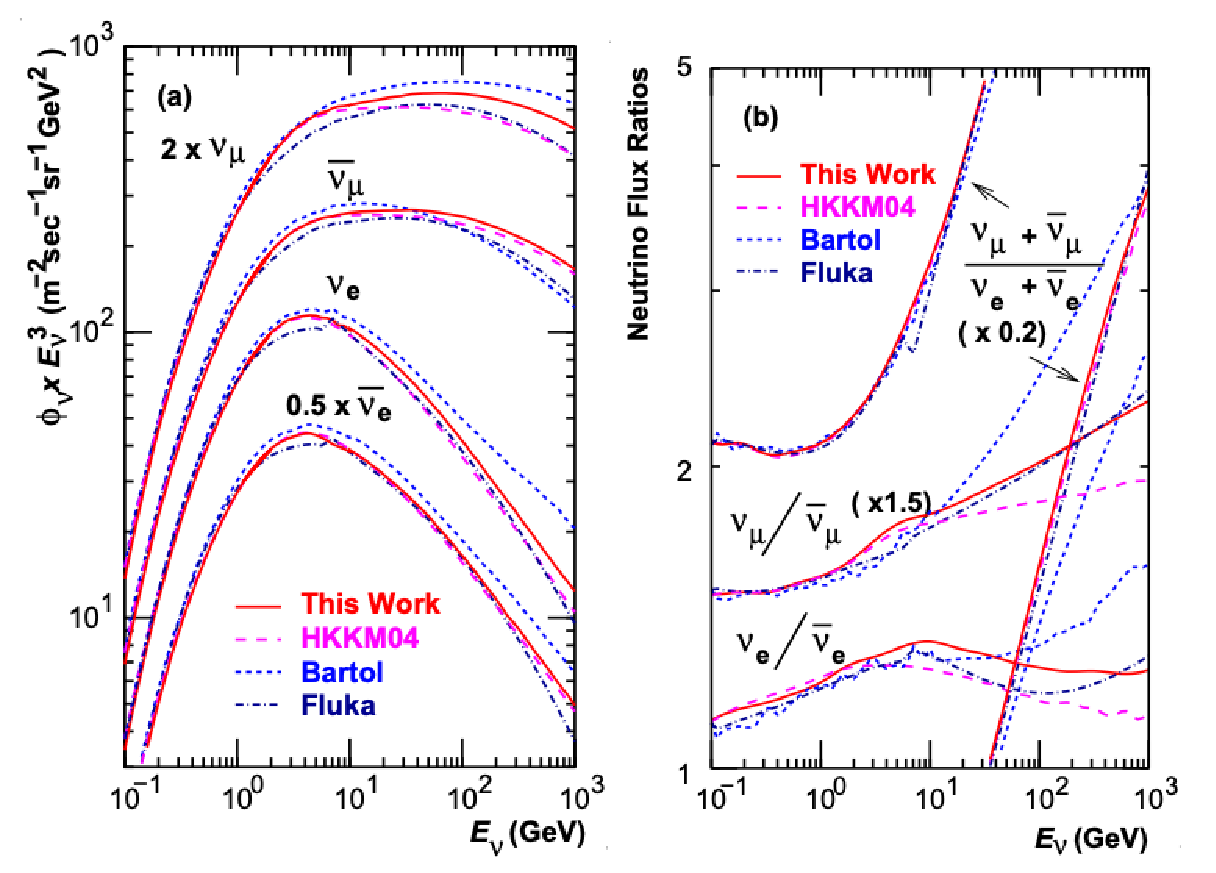
\includegraphics[width=\textwidth, trim={0mm 0mm 0mm 0mm}, clip,page=1]{Figures/Theory/AtmosphericNuFlux.pdf}
  \end{subfigure}
  \caption{Left panel: The atmospheric neutrino flux for different neutrino flavours as a function of neutrino energy as predicted by the 2007 Honda model (``This work'') \cite{Honda_2007}, the 2004 Honda model (``HKKM04'')\cite{PhysRevD.70.043008}, the Bartol model \cite{Barr_2004} and the FLUKA model \cite{etde_20239111}. Right panel: The ratio of the muon to electron neutrino flux as predicted by all the quoted models. Both figures taken from \cite{Honda_2007}.}
  \label{fig:NeutrinoOscillationPhysics_AtmosphericNeutrinoFlux}
\end{figure}

Unlike long-baseline experiments which have a fixed baseline, the distance atmospheric neutrinos propagate is dependent upon the zenith angle at which they interact. This is illustrated in \autoref{fig:NeutrinoOscillationPhysics_ZenithAngle}. Neutrinos that are generated directly above the detector (\quickmath{\cos(\theta)=1.0}) have a baseline equivalent to the height of the atmosphere whereas neutrinos that interact directly below the detector (\quickmath{\cos(\theta)=-1.0}) have to travel a length equal to the diameter of the  Earth. This means atmospheric neutrinos have a baseline that varies from \quickmath{O(20)\text{km}} to \quickmath{O(6 \times 10^{3})\text{km}}. Any neutrino generated at or below the horizon will be subject to matter effects as they propagate through the Earth.

\begin{figure}[h]
  \begin{subfigure}[t]{0.40\textwidth}
    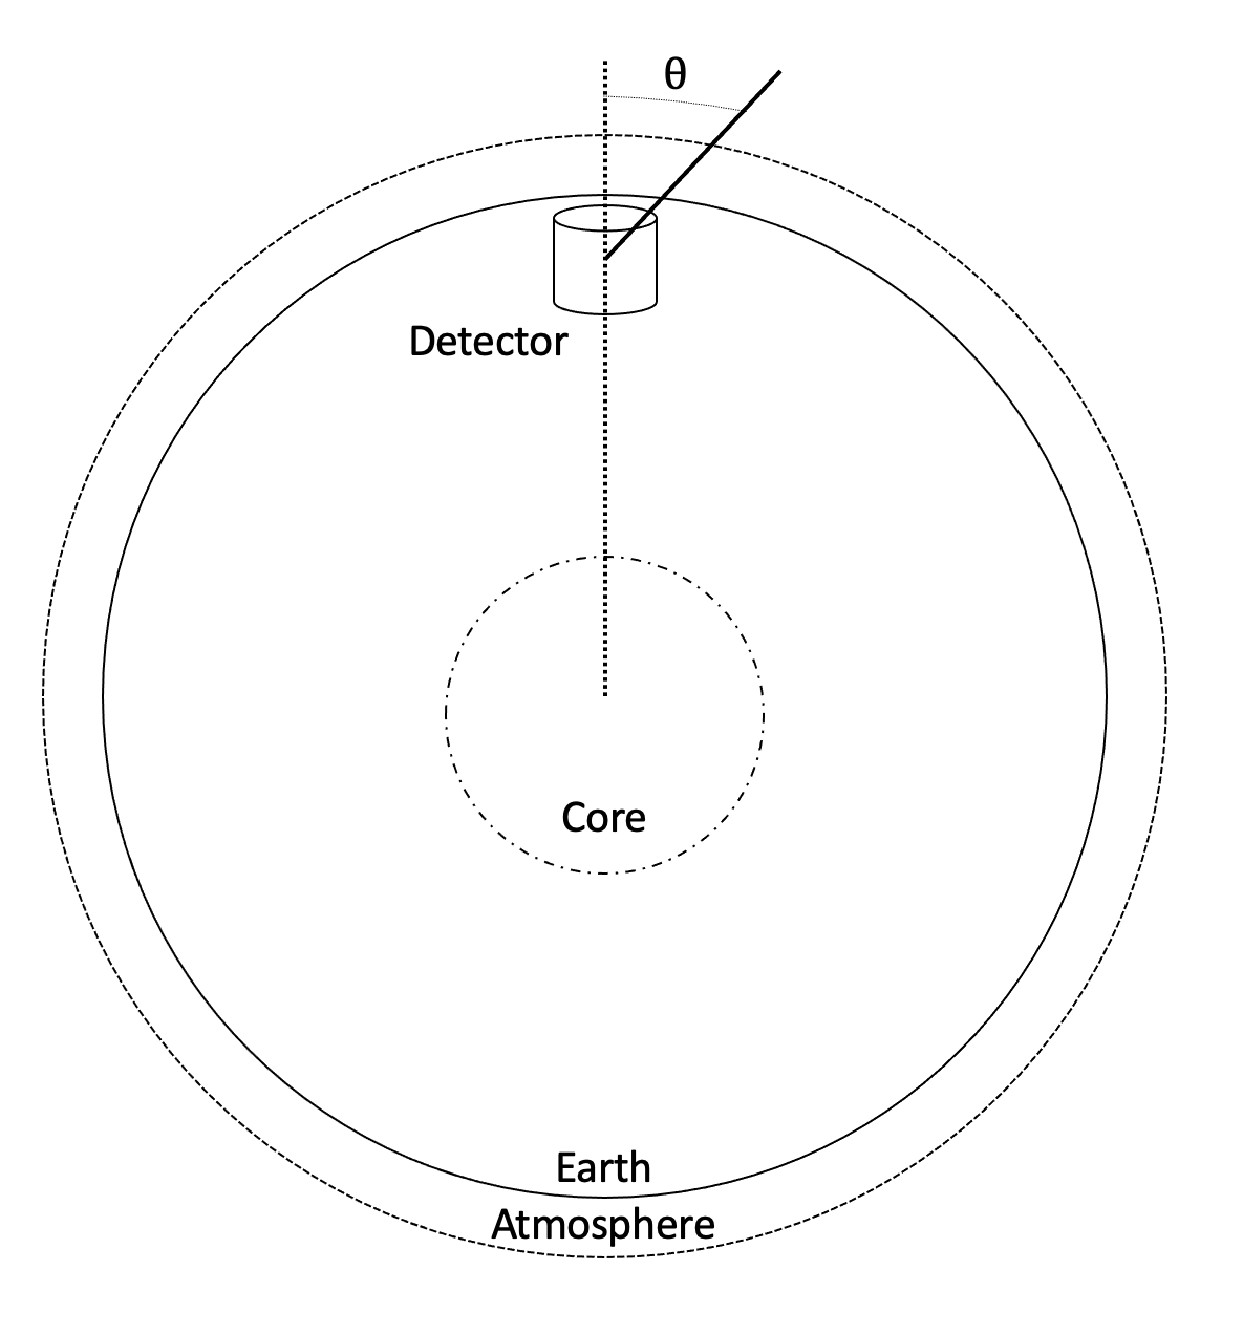
\includegraphics[width=\textwidth, trim={0mm 0mm 0mm 0mm}, clip,page=1]{Figures/Theory/ZenithAngle.pdf}
  \end{subfigure}
  \caption{A diagram illustrating the definition of zenith angle as used in the Super Kamiokande experiment \cite{Ashie_2005}.}
  \label{fig:NeutrinoOscillationPhysics_ZenithAngle}
\end{figure}

\autoref{fig:NeutrinoOscillationPhysics_NuFluxZenithAngleDep} highlights the neutrino flux as a function of the zenith angle for different slices of neutrino energy. For medium to high-energy neutrinos (and to a lesser degree for low-energy neutrinos), the flux is approximately symmetric around \quickmath{\cos(\theta)=0}. To the accuracy of this approximation, the systematic uncertainties associated with atmospheric flux for comparing upward-going and down-going neutrino cancels. This allows the down-going events, which are mostly insensitive to oscillation probabilities, to act as an unoscillated prediction (similar to a near detector in an accelerator neutrino experiment).

\begin{figure}[h]
  \begin{subfigure}[t]{0.90\textwidth}
    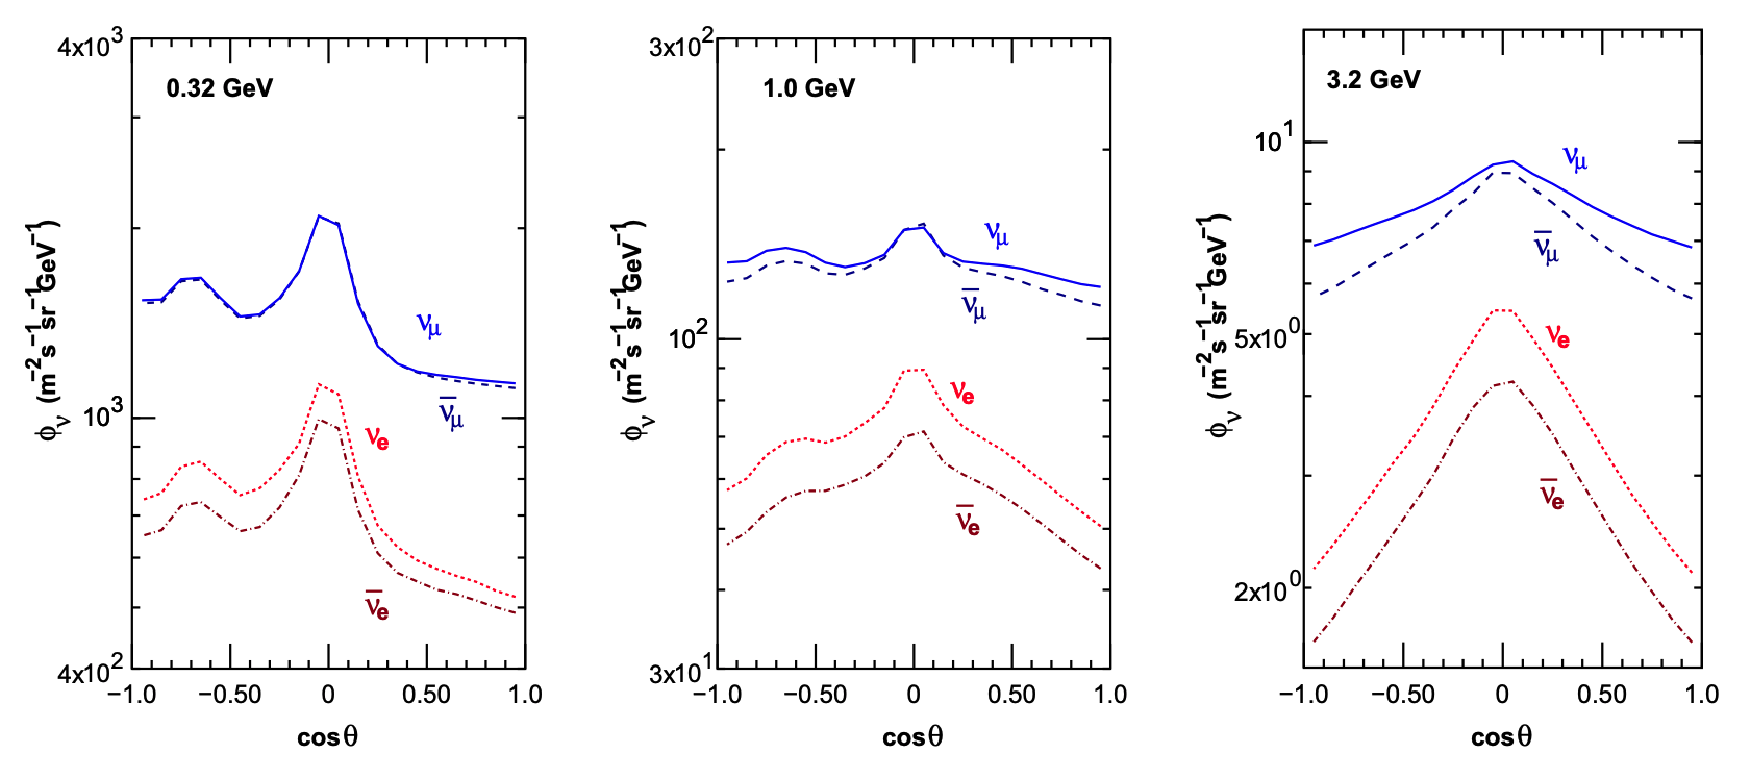
\includegraphics[width=\textwidth, trim={0mm 0mm 0mm 0mm}, clip,page=1]{Figures/Theory/NuFluxZenithAngleDep.pdf}
  \end{subfigure}
  \caption{Prediction of \quickmath{\nu_e, \bar{\nu}_{e}, \nu_{\mu}, \bar{\nu}_{\mu}} fluxes as a function of zenith angle as calculated by the HKKM model \cite{Honda:2011}. The left, middle and right panels represent three values of neutrino energy, \quickmath{0.32\text{GeV}}, \quickmath{1.0\text{GeV}} and \quickmath{3.2\text{GeV}} respectively. Predictions for other models including Bartol \cite{Barr_2004}, Honda \cite{Honda_2007} and FLUKA \cite{etde_20239111} are given in \cite{Ashie_2005}.}
  \label{fig:NeutrinoOscillationPhysics_NuFluxZenithAngleDep}
\end{figure}

Precursory hints of atmospheric neutrinos were observed in the mid-1960s searching for \quickmath{\overset{(-)}{\nu_\mu} + X \rightarrow X^{*} + \mu^{\pm}} \cite{Reines1965-cf}\ChangeOne{, although it was called an anomaly at the time of measurement}. This was succeeded with the IMB-3 \cite{PhysRevLett.66.2561} and Kamiokande \cite{Hirata1992-qz} experiments which measured the ratio of muon neutrinos compared to electron neutrinos \quickmath{R(\nu_{\mu}/\nu_{e})}. Both experiments were found to have a consistent deficit of muon neutrinos, with \quickmath{R(\nu_{\mu}/\nu_{e}) = 0.67 \pm 0.17} and \quickmath{R(\nu_{\mu}/\nu_{e}) = 0.60 \substack{+ 0.07 \\ -0.06} \pm 0.05}. %Soudan-2 \cite{Allison1997-qz} determined similar measurements.
Super-Kamiokande (SK) \cite{Ashie_2005} extended this analysis by fitting oscillation parameters in \quickmath{P(\nu_\mu \rightarrow \nu_\tau)} which found best fit parameters \quickmath{\sin^{2}(2\theta) > 0.92} and \quickmath{1.5 \times 10^{-3} < \Delta m^{2} < 3.4 \times 10^{-3} \text{eV}^{2}}.

Since then, atmospheric neutrino experiments have been making precision measurements of the \sinsqatm and \quickmath{\Delta m^{2}_{32}} oscillation parameters.
%, and to a lesser extent the sign of \delmsqatm through the matter resonance present for any neutrinos passing through the Earth.
Atmospheric neutrino oscillation is dominated by \quickmath{P(\nu_{\mu} \rightarrow \nu_{\tau})}, where SK observed a \quickmath{4.6\sigma} discovery of \quickmath{\nu_{\tau}} appearance \cite{Li_2018}. \autoref{fig:NeutrinoOscillationPhysics_AtmosphericParamContour} illustrates the current estimates on the atmospheric mixing parameters from a wide range of atmospheric and accelerator neutrino observatories.

\begin{figure}[h]
  \begin{subfigure}[t]{0.90\textwidth}
    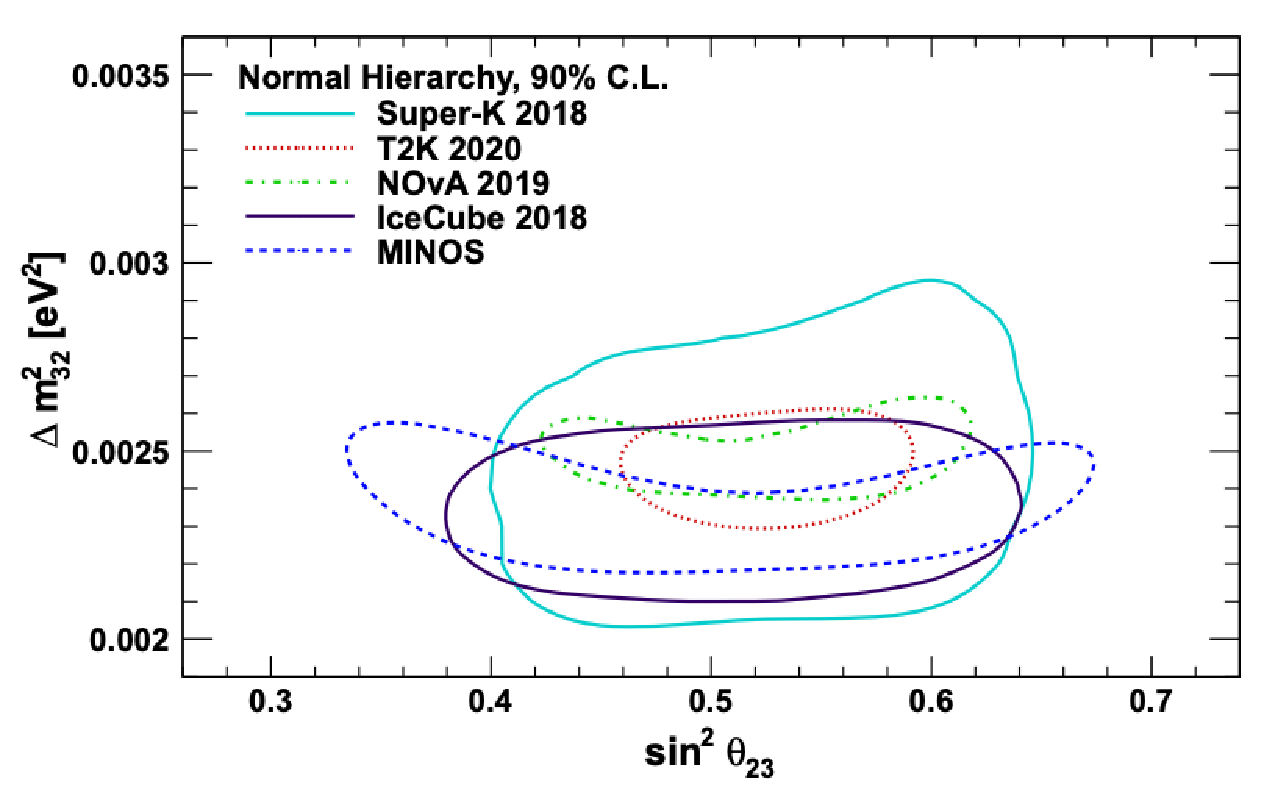
\includegraphics[width=\textwidth, trim={0mm 0mm 0mm 0mm}, clip,page=1]{Figures/Theory/AtmosphericParams.pdf}
  \end{subfigure}
  \caption{Constraints on the atmospheric oscillation parameters, \sinsqatm and \delmsqatm, from atmospheric and long baseline experiments: SK \cite{Kamiokande_Collaboration2017-nf}, T2K \cite{T2K_Collaboration2018-sm}, \quickmath{\text{NO}\nu\text{A}} \cite{Acero2019-rw}, IceCube \cite{Aartsen2018-cz} and MINOS \cite{Adamson2014-tt}. Figure taken from \cite{Athar_2022}.}
  \label{fig:NeutrinoOscillationPhysics_AtmosphericParamContour}
\end{figure}

\subsection{Accelerator Neutrinos}
\label{subsec:NeutrinoOscillationPhysics_AcceleratorNeutrinos}

The concept of using a man-made ``neutrino beam'' was first realised in 1962 \cite{Danby1962-ph}.
%and led to the first discovery that \quickmath{\nu_{e}} and \quickmath{\nu_{\mu}} were in fact different particles.
Since then, many experiments have followed which all use the same fundamental concepts. Typically, a proton beam is aimed at a target producing charged mesons that decay to neutrinos. The mesons can be sign-selected by the use of magnetic focusing horns to generate a neutrino or antineutrino beam.
%Absorbing material and the rock between the target and detector absorb all particles barring the neutrinos.
Pions are the primary meson that decay and depending on the orientation of the magnetic field, a muon (anti-)neutrino beam is generated via \quickmath{\pi^{+} \rightarrow \mu^{+} + \nu_{\mu}} or \quickmath{\pi^{-} \rightarrow \mu^{-} + \bar{\nu}_{\mu}}. The decay of muons and kaons does result in an irreducible intrinsic electron neutrino background. In T2K, this background contamination is \quickmath{O(<1\%)} \cite{Abe_2013}. There is also an approximately \quickmath{\sim 5\%} ``wrong-sign'' neutrino background of \quickmath{\bar{\nu}_{\mu}} generated via the same decays. \ChangeOne{As the beam is generated by proton interactions (rather than anti-proton interactions), the wrong-sign component in the antineutrino beam is larger when operating in neutrino mode.}

\ChangeOneRM{The energy of each neutrino in the beam is dependent on the energy of the initial proton beam. Therefore, tuning the proton energy allows} \ChangeOne{Tuning the proton energy in the beam and using beam focusing techniques allows} the neutrino energy to be set to a value that maximises the disappearance oscillation probability in the \quickmath{L/E} term in \autoref{eq:NeutrinoOscillationPhysics_PMNS_2FlavourOscProb}.
%As the inital proton beam can be tuned resulting in a tunable neutrino energy spectra, the advantage of these type of experiments is that they can be focused in on the oscillation dip presented by the \quickmath{L/E} term in \autoref{eq:NeutrinoOscillationPhysics_PMNS_2FlavourOscProb} using the two flavour approximation.
This means that accelerator experiments are typically more sensitive to the mixing parameters as compared to a natural neutrino source. However, the disadvantage compared to atmospheric neutrino experiments is that the baseline has to be shorter due to the lower flux. Consequently, there is typically less sensitivity to matter effects and the ordering of the neutrino mass eigenstates.

A neutrino experiment measures

\begin{equation}
  \label{eq:NeutrinoOscillationPhysics_DetectorMeasurement}
  R(\vec{x}) = \Phi(E_{\nu}) \times \sigma(E_{\nu}) \times \epsilon(\vec{x}) \times P(\nu_{\alpha} \rightarrow \nu_{\beta}),
\end{equation}

where \quickmath{R(\vec{x})} is the event rate of neutrinos at position \quickmath{\vec{x}}, \quickmath{\Phi(E_{\nu})} is the flux of neutrinos with energy \quickmath{E_{\nu}}, \quickmath{\sigma(E_{\nu})} is the cross-section of the neutrino interaction and \quickmath{\epsilon(\vec{x})} is the efficiency \ChangeOne{and resolution} of the detector. In order to leverage the most out of an accelerator neutrino experiment, the flux and cross-section systematics need to be constrained. This is typically done via the use of a ``near detector'', situated at a baseline of \quickmath{O(1)\text{km}}. This detector observes the unoscillated neutrino flux and constrains the parameters used within the flux and cross-section model.

The first accelerator experiments to precisely measure oscillation parameters were MINOS \cite{PhysRevLett.97.191801} and K2K \cite{PhysRevLett.9.36}.
These experiments confirmed the \ChangeOneRM{$\nu_{\mu} \rightarrow \nu_{\mu}$ oscillations} \ChangeOne{\quickmath{\nu_{\mu}} disappearance} seen in atmospheric neutrino experiments by finding consistent \ChangeOneRM{mixing} parameter values for \sinsqatm and \delmsqatm.
The current generation of accelerator neutrino experiments, T2K and \NOVA extended this field by observing \quickmath{\bar{\nu}_{\mu} \rightarrow \bar{\nu}_{e}} and lead the sensitivity to atmospheric mixing parameters as seen in \autoref{fig:NeutrinoOscillationPhysics_AtmosphericParamContour} \cite{PhysRevLett.123.151803}.
The two experiments differ in their peak neutrino energy, baseline, and detection technique.
The \NOVA experiment is situated at a baseline of \quickmath{810\text{km}} from the NuMI beamline which delivers \quickmath{2\text{GeV}} neutrinos.
The T2K neutrino beam is peaked around \quickmath{0.6 \text{GeV}} and propagates \quickmath{295\text{km}}.
The \NOVA experiment also uses functionally identical detectors (near and far) which allow the approximate cancellation of detector systematics whereas T2K uses a plastic scintillator technique at the near detector and a water Cherenkov far detector.
The future generation experiments DUNE \cite{Abi2020-cm} and Hyper-Kamiokande \cite{Hyper-Kamiokande_Proto-Collaboration2015-ac} will succeed these experiments as the high-precision era of neutrino oscillation parameter measurements develops.

Several anomalous results have been observed in the LSND \cite{PhysRevD.64.112007} and MiniBooNE \cite{PhysRevLett.110.161801} detectors which were designed with purposefully short baselines. Parts of the neutrino community attributed these results to oscillations induced by a fourth ``sterile'' neutrino \cite{Blanco_2020} but several searches in other experiments, MicroBooNE \cite{10.48550/arxiv.2110.14054} and KARMEN \cite{PhysRevD.65.112001}, found no hints of additional neutrino species. The solution to the anomalous results \ChangeOneRM{are} \ChangeOne{is} still being determined.

\subsection{Reactor Neutrinos}
\label{subsec:NeutrinoOscillationPhysics_ReactorNeutrinos}

As illustrated in the first discovery of neutrinos (\autoref{sec:NeutrinoOscillationPhysics_Discovery}), nuclear reactors are a very useful man-made source of electron antineutrinos. For reactors that use low-enriched uranium \quickmath{^{235}\text{U}} as fuel, the antineutrino flux is dominated by the \quickmath{\beta}-decay fission of \quickmath{^{235}\text{U}}, \quickmath{^{238}\text{U}}, \quickmath{^{239}\text{Pu}} and \quickmath{^{241}\text{Pu}} \cite{Kim2013-ye} as illustrated in \autoref{fig:NeutrinoOscillationPhysics_ReactorNeutrinoProduction}.

\begin{figure}[h]
  \begin{subfigure}[t]{0.90\textwidth}
    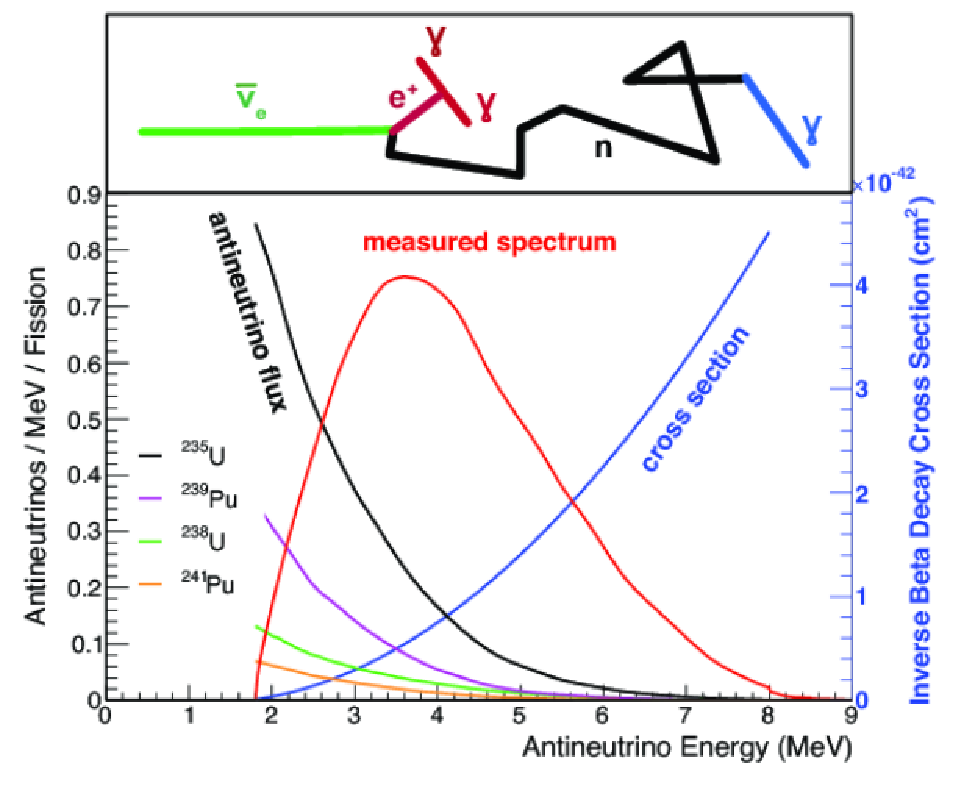
\includegraphics[width=\textwidth, trim={0mm 0mm 0mm 0mm}, clip,page=1]{Figures/Theory/ReactorNeutrinoProduction.pdf}
  \end{subfigure}
  \caption{Reactor electron antineutrino fluxes for \quickmath{^{235}\text{U}} (Black), \quickmath{^{238}\text{U}} (Green), \quickmath{^{239}\text{Pu}} (Purple), and \quickmath{^{241}\text{Pu}} (Orange) isotopes. The inverse \quickmath{\beta}-decay cross-section (Blue) and corresponding measurable neutrino spectrum (Red) are also given. Top panel: Schematic of Inverse \quickmath{\beta}-decay interaction including the eventual capture of the emitted neutron. This capture emits a \quickmath{\gamma}-ray which provides a second signal of the event. Taken from \cite{SajjadAthar:2021prg}.}
  \label{fig:NeutrinoOscillationPhysics_ReactorNeutrinoProduction}
\end{figure}

Due to their low energy, reactor electron antineutrinos predominantly interact via the inverse \quickmath{\beta}-decay (IBD) interaction. The typical signature contains two signals delayed by \quickmath{O(200)\mu\text{s}}; firstly the prompt photons from positron annihilation, and secondly the photons emitted (\quickmath{E_{tot}^{\gamma} = 2.2\text{MeV}}) from de-excitation after neutron capture on hydrogen. Searching for both signals improves the detector's ability to distinguish between background and signal events \cite{Abe2022-ij}. Recently, SK included gadolinium dopants into the ultra-pure water to increase the energy released from the photon cascade to \quickmath{\sim 8\text{MeV}} and reduce the time of the delayed signal to \quickmath{\sim 28 \mu \text{s}}.

There are many short baseline experiments (\quickmath{\text{L} \sim O(1)\text{km}}) that have measured the \sinsqreac and \delmsqatm oscillation parameters. Daya Bay \cite{PhysRevLett.108.171803}, RENO \cite{PhysRevLett.108.191802} and Double Chooz \cite{PhysRevLett.108.131801} have all provided precise measurements, with the first discovery of a non-zero \quickmath{\theta_{13}} made by Daya Bay and RENO (and \ChangeOneRM{complimented} \ChangeOne{complemented} by T2K \cite{PhysRevLett.108.131801}). The constraints on \sinsqreac by the reactor experiments lead the field and are often used as external inputs to accelerator neutrino experiments to improve their sensitivity to \dcp and mass hierarchy determination.
%One curiosity of these short baseline reactor experiments is the `\quickmath{5 \text{MeV}} excess' \cite{Berryman_2019}. First observed in 2014 \cite{For_the_RENO_Collaboration2015-zy, Abe_2014}, all three experiments listed observed a shape excess in events around \quickmath{E_{\nu} \sim 5 \text{MeV}}. The reason behind this excess is speculated to be either oscillations to sterile neutrinos or a fault in the Huber-Mueller model \cite{Mueller_2011}. At this time, the latter is favoured as Daya Bay \cite{PhysRevLett.123.111801} observed substantial evidence (\quickmath{4.0\sigma}) of correlation between the excess and the \quickmath{^{235}\text{U}} electron antineutrino flux.
%Other neutrino experiments, PROSPECT \cite{PhysRevD.103.032001} and STEREO \cite{STEREO} show similar results data to help determine the cause of the excess.
JUNO-TAO \cite{junocollaboration2020tao}, a small collaboration within the larger JUNO experiment, is a next-generation reactor experiment that aims to precisely measure the isotopic antineutrino yields from the different fission chains. Alongside this, it aims to explain the `\quickmath{5 \text{MeV}} excess' \cite{For_the_RENO_Collaboration2015-zy, Abe_2014, PhysRevLett.123.111801} by conducting a search for sterile neutrinos with a mass scale of around \quickmath{1 \text{eV}}.

Kamland \cite{Decowski2016-hh} is the only experiment to have observed reactor neutrinos using a long baseline (flux weighted averaged baseline of \quickmath{L \sim 180\text{km}}) which allows it to have sensitivity to \delmsqsol. Combined with the SK solar neutrino experiment, the combined analysis puts the most stringent constraint on \delmsqsol \cite{PhysRevD.83.052002} \ChangeOneRM{which is used as a prior uncertainty within accelerator neutrino experiments}.

\section{Summary}
\label{sec:Theory_Summary}

Since observing the first evidence of neutrino oscillations in the late 1990's, numerous measurements of the mixing parameters have been made. Many experiments use neutrinos as a tool for discovery of new physics (diffuse supernoave background, neutrinoless double beta decay and others) so the PMNS parameters are summarised in the Particle Data Group (PDG) review tables. The analysis presented in this thesis focuses on the 2020 T2K oscillation analysis presented in \cite{Dunne2020-uf} where the 2018 PDG constraints \cite{Tanabashi2018-hp} were used. These constraints are outlined in \autoref{tab:Theory_PDGConstraints}.

\begin{table}[ht!]
    \centering
    \begin{tabular}{c|c}
      \hline
      Parameter & 2018 Constraint \\
      \hline
      \quickmath{\sin^{2}(\theta_{12})} & \quickmath{0.307 \pm 0.013} \\
      \quickmath{\Delta m^{2}_{21}} & \quickmath{(7.53 \pm 0.18) \times 10^{-5} \text{eV}^{2}} \\
      \quickmath{\sin^{2}(\theta_{13})} & \quickmath{(2.12 \pm 0.08) \times 10^{-2}} \\
      \quickmath{\sin^{2}(\theta_{23})} (I.H., Q1) & \quickmath{0.421^{+0.033}_{-0.025}} \\
      \quickmath{\sin^{2}(\theta_{23})} (I.H., Q2) & \quickmath{0.592^{+0.023}_{-0.030}} \\
      \quickmath{\sin^{2}(\theta_{23})} (N.H., Q1) & \quickmath{0.417^{+0.025}_{-0.028}} \\
      \quickmath{\sin^{2}(\theta_{23})} (N.H., Q2) & \quickmath{0.597^{+0.024}_{-0.030}} \\
      \quickmath{\Delta m^{2}_{32}} (I.H.) & \quickmath{(-2.56 \pm 0.04) \times 10^{-3} \text{eV}^{2}} \\
      \quickmath{\Delta m^{2}_{32}} (N.H.) & \quickmath{(2.51 \pm 0.05) \times 10^{-3} \text{eV}^{2}} \\
      \hline
      \hline
    \end{tabular}
    \caption{The 2018 Particle Data Group constraints of the oscillation parameters taken from \cite{Tanabashi2018-hp}. The value of \delmsqatm is given for both normal hierarchy (N.H.) and inverted hierarchy (I.H.) and \sinsqatm is broken down by whether its value is below (Q1) or above (Q2) \quickmath{0.5}.}
    \label{tab:Theory_PDGConstraints}
\end{table}

The \sinsqreac measurement stems from the electron antineutrino disappearance, \quickmath{P(\bar{\nu}_{e} \rightarrow \bar{\nu}_{e})}, and is take as the  average best-fit from the combination of Daya Bay, Reno and Double Chooz. It is often used as a prior uncertainty within other neutrino oscillation experiments, typically termed the reactor constraint. The \sinsqsol parameter is predominantely measured through electron neutrino disappearance, \quickmath{P(\nu_{e} \rightarrow \nu_{\mu,\tau})}, in solar neutrino experiments. The long-baseline reactor neutrino experiment Kamland also has sensitivity to this parameter and is used in a joint fit to solar data from SNO and SK, using the reactor constraint. Measurements of \sinsqatm are made by long-baseline and atmospheric neutrino experiments. The PDG value is a joint fit of T2K, \NOVA, MINOS and IceCube DeepCore experiments. The latest T2K-only meaurement, provided at Neutrino2020 and is the basis of this thesis, is given as \quickmath{\sin^{2}(\theta_{23}) = 0.546^{+0.024}_{-0.046}} \cite{Dunne2020-uf}. The PDG constraint on \delmsqsol is provided by the KamLAND experiment using solar and geoneutrino data. This measurement utilised a \sinsqreac constraint from accelerator (T2K, MINOS) and reactor neutrino (Daya Bay, RENO, Double Chooz) experiments. Accelerator measurements make some of the most stringent constraints on \delmsqatm although atmospheric experiments have more sensitivity to the mass hierarchy determination. The PDG performs a joint fit of accelerator and atmospheric data, in both normal and inverted hierarchy separately. The latest T2K-only result is \quickmath{\Delta m^{2}_{32} = 2.49^{+0.058}_{-0.082} \times 10^{-3}\text{eV}^{2}} favouring normal hierarchy \cite{Dunne2020-uf}. The value of \dcp is largely undetermined. CP-conserving values of \quickmath{0} and \quickmath{\pi} were rejected with \quickmath{\sim 2\sigma} intervals, as published in Nature, although more recent analysis have reduced the rejection intervals to \quickmath{90\%}. Since the 2018 PDG publication, there has been a new measurement of \quickmath{\sin^{2}(\theta_{13}) = (2.20 \pm 0.07) \times 10^{-2}} \cite{Workman:2022ynf}, alongside updated \delmsqatm and \sinsqatm measurements.

Throughout this thesis, several sample spectra predictions and contours are presented which require oscillation parameters to be assumed. \autoref{tab:Theory_ParameterSets} defines two sets of oscillation parameters, with ``Asimov A'' set being close to the preferred values from a previous T2K-only fit \cite{PhysRevLett.112.181801} and ``Asimov B'' being CP-conserving and further from maximal \quickmath{\theta_{23}} mixing.

\begin{table}[ht!]
    \centering
    \begin{tabular}{c|c|c}
      \hline
      \hline
      Parameter & Asimov A & Asimov B \\
      \hline
      \quickmath{\Delta m^{2}_{12}} & \multicolumn{2}{c}{\quickmath{7.53 \times 10^{-5} \text{eV}^{2}}} \\ \hline
      \quickmath{\Delta m^{2}_{32}} & \multicolumn{2}{c}{\quickmath{2.509 \times 10^{-3} \text{eV}^{2}}} \\ \hline
      \quickmath{\sin^{2}\left(\theta_{12}\right)} & \multicolumn{2}{c}{\quickmath{0.304}} \\ \hline
      \quickmath{\sin^{2}\left(\theta_{13}\right)} & \multicolumn{2}{c}{\quickmath{0.0219}} \\ \hline
      \quickmath{\sin^{2}\left(\theta_{23}\right)} & \quickmath{0.528} & \quickmath{0.45} \\ \hline
      \quickmath{\delta_{CP}} & \quickmath{-1.601} & \quickmath{0.0} \\ \hline
      \hline
    \end{tabular}
    \caption{Reference values of the neutrino oscillation parameters for two different oscillation parameter sets.}
    \label{tab:Theory_ParameterSets}
\end{table}
